% !TEX root = main.tex

\section{图像分割} % Chap 10
图像分割一般基于亮度值的两种基本特性(\textbf{不连续性}和\textbf{相似性})来分割。

\begin{definition}[分割]
令$R$为全图,可将分割看作$R$划分为$n$个子区域$R_1,R_2,\ldots,R_n$的过程:
\begin{enumerate}
	\item $\disp\bigcup_{i=1}^n R_i=R$
	\item $R_i$是一个连通区域
	\item $R_i\cap R_j=\varnothing$
	\item $Q(R_i)=TRUE$
	\item $Q(R_i\cup R_j)=FALSE$,对于任何$R_i$和$R_j$的邻接区域
\end{enumerate}
其中,$Q(R_k)$为定义在集合$R_k$的点上的逻辑属性
\end{definition}

\subsection{点检测与线检测}
\subsubsection{点检测}
\begin{center}
\begin{tabular}{|c|c|c|}\hline
1 & 1 & 1\\\hline
1 & -8 & 1\\\hline
1 & 1 & 1\\\hline
\end{tabular}
\end{center}
若作用算子后的图像$|R(x,y)|\geq T$,则记为$1$。

\subsubsection{线检测}
\begin{figure}[H]
\centering
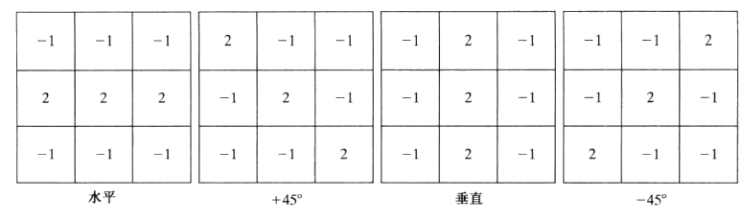
\includegraphics[width=0.9\linewidth]{fig/line_detect.png}
\end{figure}

\subsection{边缘检测}
傅里叶变换无法刻画边缘,只知道高频成分,不知道高频在哪里。
一种方法是局部傅里叶变换,衍生出小波变换(就是要构造一种高通滤波器):有震荡信号的位置(小范围震荡且积分为0),可以刻画边缘。

台阶/阶梯、斜坡/斜、屋顶/Delta边缘模型如下。
\begin{figure}[H]
\centering
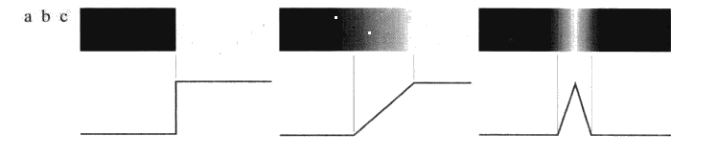
\includegraphics[width=0.9\linewidth]{fig/edge_model.png}
\end{figure}

如下图所示,二阶导数会增大噪声,因此做边缘检测之前应该先抑制噪声(平滑)。
\begin{figure}[H]
\centering
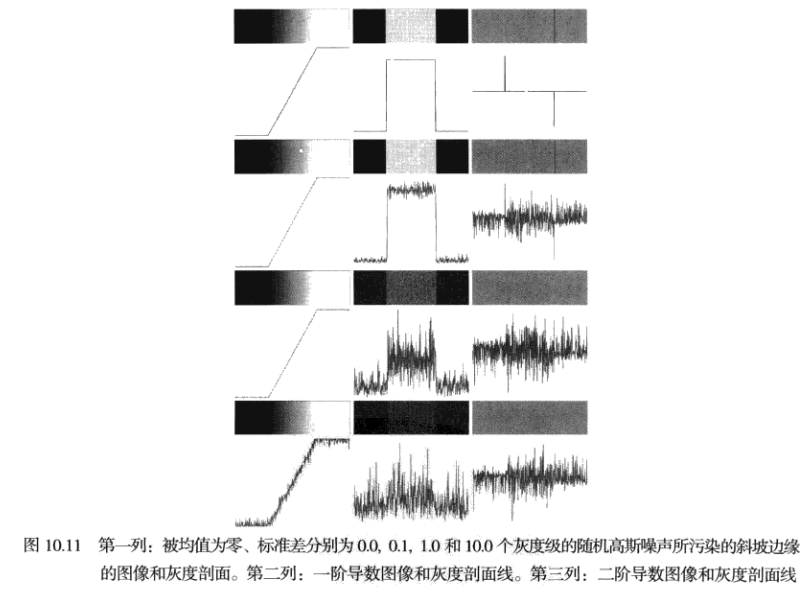
\includegraphics[width=0.9\linewidth]{fig/edge_detect_noise.png}
\end{figure}

常用的边缘检测算子:一阶微分-梯度,二阶微分-Laplace算子
\begin{figure}[H]
\centering
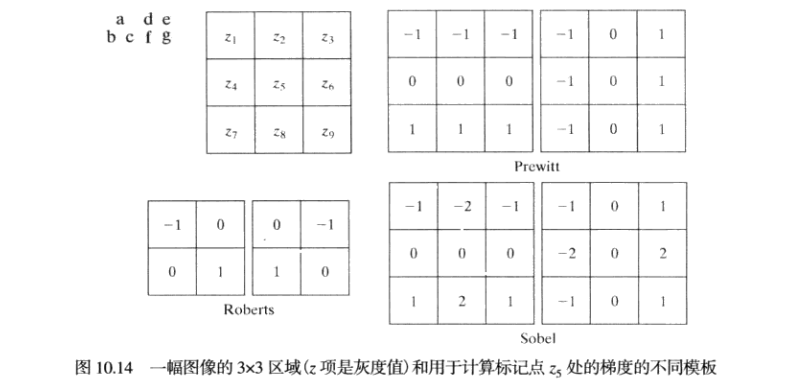
\includegraphics[width=0.9\linewidth]{fig/edge_detect_op.png}
\end{figure}

\subsubsection{Marr-Hildreth边缘检测器}
由于拉普拉斯算子的应用通常会放大图像的噪声,因此通常先平滑,再应用拉普拉斯算子。
假设$f(x,y)$为图像,$h(x,y)$为高斯平滑函数
\[h(x,y)=-\ee^{-\frac{x^2+y^2}{2\sigma^2}}\]
则只需做一步操作完成平滑及边缘检测
\[\nabla^2 [f(x,y)*h(x,y)]=f(x,y)*[\nabla^2 h(x,y)]\]
其中
\[\nabla^2 h(x,y)=\frac{2}{\sigma^2}\lrs{1-\frac{x^2+y^2}{2\sigma^2}}\ee^{-\frac{x^2+y^2}{2\sigma^2}}\]
即高斯拉普拉斯(LoG)变换。

墨西哥草帽函数。
(高斯函数的微分就是一种小波,做微分后负号与负号抵消;而且高斯函数有无穷阶导数)
\begin{figure}[H]
\centering
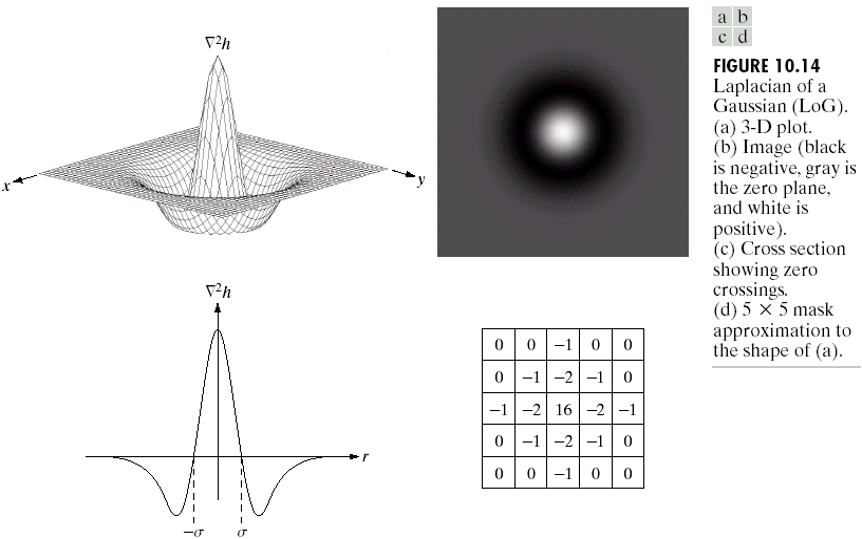
\includegraphics[width=0.6\linewidth]{fig/LoG.png}
\end{figure}

得到Marr-Hildreth的边缘检测算法
\begin{enumerate}
	\item 计算高斯拉普拉斯变换(LoG)
	\item 找到零交叉点(边缘正负变化的地方)
\end{enumerate}

用高斯差分DoG滤波可以近似代替LoG,
\[DoG(x,y)=\frac{1}{2\pi\sigma_1^2}\ee^{-\frac{x^2+y^2}{2\sigma_1^2}}-\frac{1}{2\pi\sigma_2^2}\ee^{-\frac{x^2+y^2}{2\sigma_2^2}},\;\sigma_1>\sigma_2\]
以$\sigma_1:\sigma_2=1.6:1$来定,则近似的$\sigma$为
\[\sigma^2=\frac{\sigma_1^2\sigma_2^2}{\sigma_1^2-\sigma_2^2}\ln\lrs{\frac{\sigma_1^2}{\sigma_2^2}}\]

\subsubsection{Canny边缘检测器}
目标:
\begin{itemize}
	\item 低错误率:边缘一个不落,一个不多
	\item 边缘点应该被很好定位:标记的边缘点与真实边缘中心之间的距离最小
	\item 单一边缘点响应:对于真实的边缘点,检测器仅返回一个点,即真实边缘周围的局部最大数应该最小
\end{itemize}

算法步骤:
\begin{enumerate}
	\item 用一个高斯滤波器平滑输入图像
	\item 计算梯度幅值图像和角度图像(Canny为二阶梯度算子)
	\[M(x,y)=\sqrt{g_x^2+g_y^2},\quad\alpha(x,y)=\arctan\lrs{\frac{g_y}{g_x}}\]
	\item 对梯度幅值图像应用非最大抑制
\begin{figure}[H]
\centering
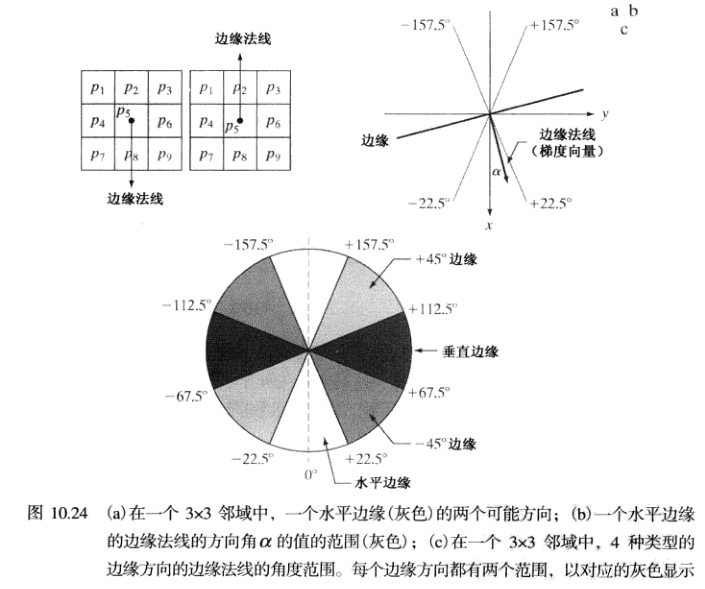
\includegraphics[width=0.6\linewidth]{fig/canny-margin.png}
\end{figure}
\begin{enumerate}
	\item 寻找最接近$\alpha(x,y)$的方向$d$
	\item $g_N$代表细化后的边缘
	\[g_N(x,y)=\begin{cases}0 & M(x,y)\text{的值至少小于沿$d$的两个邻居之一}\\M(x,y) & \text{否则}\end{cases}\]
\end{enumerate}
	\item 用双阈值处理和连接分析来检测并连接边缘\\
	双阈值法:高阈值$T_H$和低阈值$T_L$,比率为$2:1$或$3:1$
	\[\begin{aligned}
	g_{NN}(x,y) &= g_N(x,y)\geq T_H & \text{强边缘}\\
	g_{NL}(x,y) &= g_N(x,y)\geq T_L & \text{弱边缘(可能是边缘也可能不是)+强边缘}\\
	g_{NL}(x,y) &= g_{NL}(x,y)-g_{NH}(x,y) & \text{弱边缘}
	\end{aligned}\]
	用弱边缘补齐强边缘来获得完整边缘
\begin{enumerate}
	\item 在$g_{NN}(x,y)$中定位下一个未被访问的边缘像素$p$
	\item 在$g_{NL}(x,y)$中用8连通方法连接到$p$
	\item 如果$g_{NN}(x,y)$中所有非零标记都已经访问过,则跳到(d),否则(a)
	\item 将$g_{NL}(x,y)$中未被标记为有效边缘的像素的所有像素置零。
	将$g_{NL}(x,y)$中非零像素附加到$g_{NN}(x,y)$
\end{enumerate}
\end{enumerate}

\subsection{边缘连接}
\textbf{边界是封闭的边缘。}
\[\text{边界检测}=\text{边缘检测}+\text{边缘连接}\]

\begin{itemize}
\item 边缘连接:两个端点只有在边缘强度和走向相近的情况下才能连接。
如果像素$(s,t)$在像素$(x,y)$的邻域内且满足:
\[|M(x,y)-M(s,t)|\leq E,\quad |\alpha(x,y)-\alpha(s,t)|\leq A\]
则可以将$(s,t)$与$(x,y)$连接起来。

\item 边界跟踪:依照角度搜索,用$3\times 3$区域平均值代替单像素点(避免噪声影响),称为虫
\begin{figure}[H]
\centering
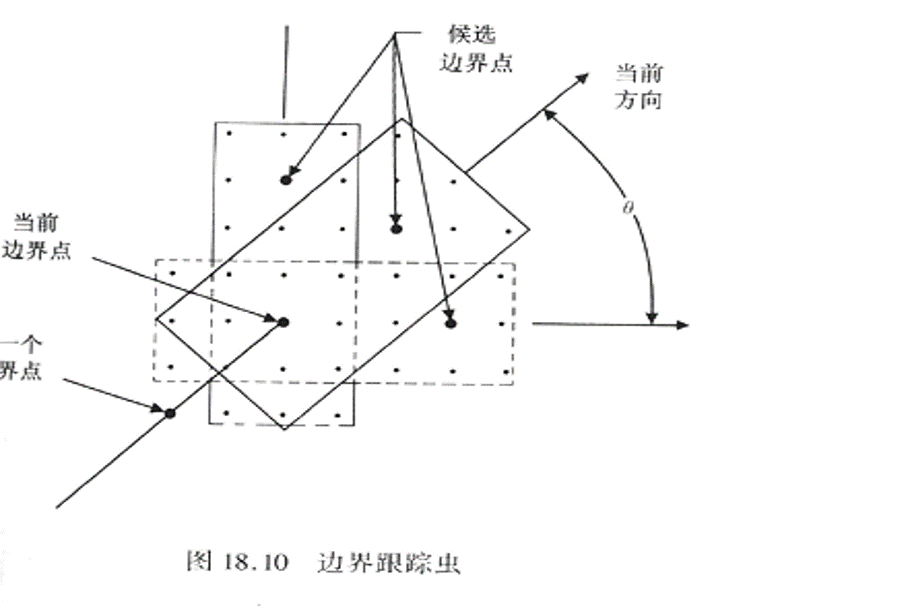
\includegraphics[width=0.5\linewidth]{fig/boundary_tracing.png}
\end{figure}

\item 区域处理:用多边形拟合算法
\begin{figure}[H]
\centering
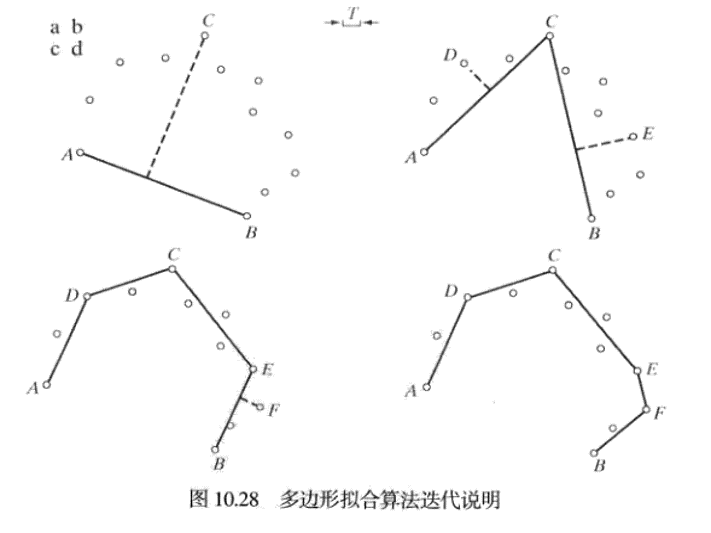
\includegraphics[width=0.5\linewidth]{fig/polygon_boundary.png}
\end{figure}
\end{itemize}

\subsection{边界检测}
用Hough变换进行边界检测:通过边界点找已知形状的目标。 % 考试必考

\subsubsection{直线检测问题}
已知一组边缘点,找一条直线,使它通过最多边缘点。

直线方程用极坐标表示
\[\rho=x\cos\theta+y\sin\theta\]
通过辅助角变换可得
\[\rho=A_0\sin(\theta+\phi_0)\]
故可映射到$\rho O\theta$空间,其中每一个点是$xOy$平面上的通过同一个点的一条线。
\begin{figure}[H]
\centering
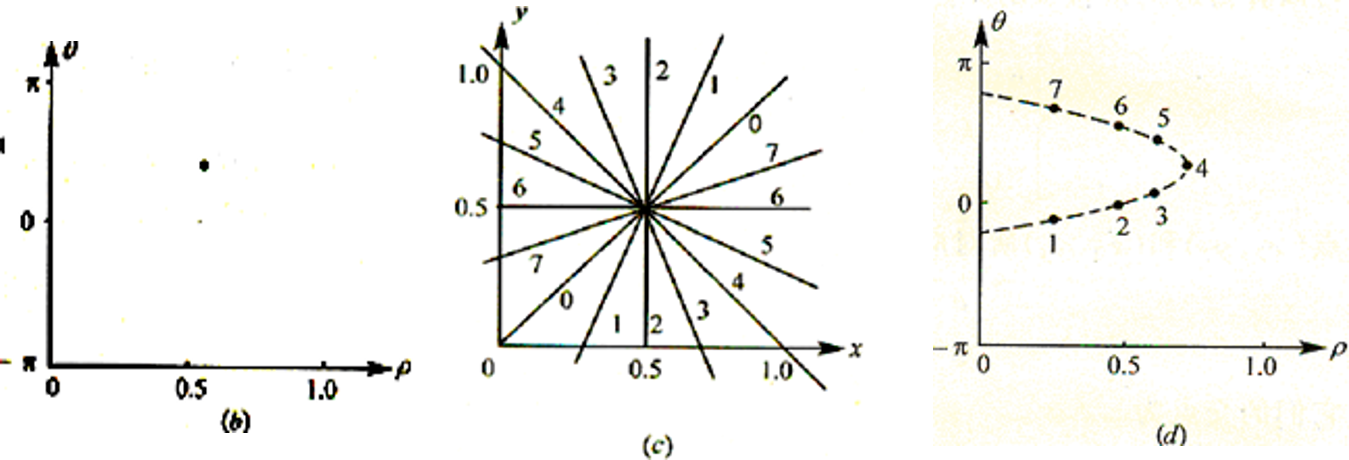
\includegraphics[width=0.6\linewidth]{fig/hough.png}
\end{figure}

如果有一组位于由参数$\rho_0$和$\theta_0$决定的直线上的边缘点,则每个边缘点对应了$\rho,\theta$空间的一条正弦曲线。
所有这些曲线必然会交于点$(\rho_0,\theta_0)$,因为这是它们共享的一条直线的参数。
\begin{figure}[H]
\centering
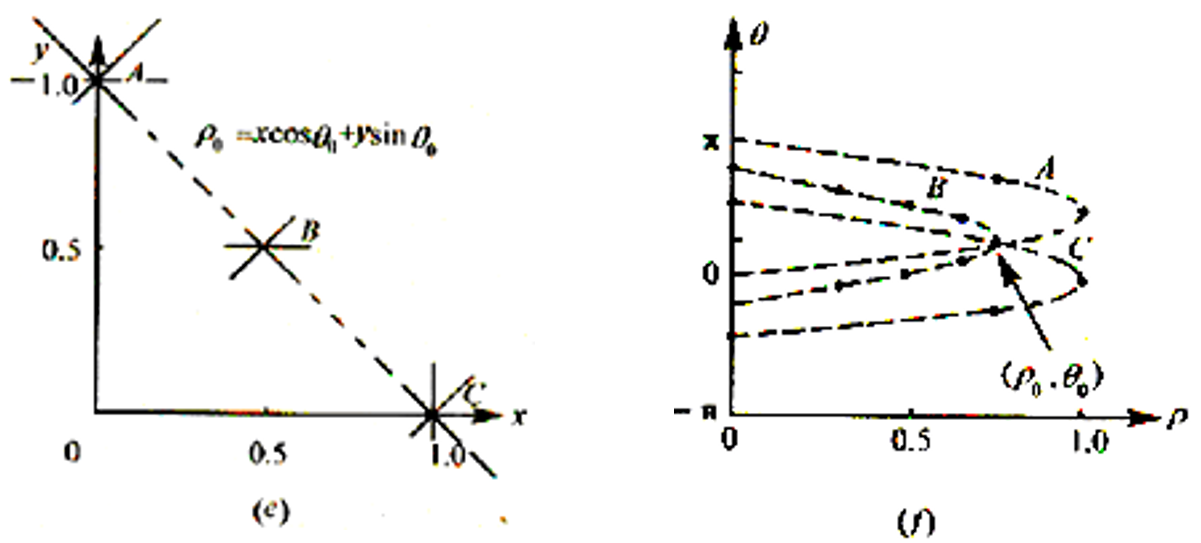
\includegraphics[width=0.6\linewidth]{fig/hough2.png}
\end{figure}

故对于边缘点的直线拟合问题,即找一个使边缘点确定的正弦曲线相交最多的点$(\rho,\theta)$。

可以建立$\rho,\theta$空间的二维直方图来确定对于边缘点的最佳拟合直线参数$(\rho_0,\theta_0)$。
具体算法如下:
\begin{enumerate}
	\item 对于每个边缘点$(x,y)$。建立直线方程:
	\[\rho=x\cos(\theta)+y\sin(\theta)\]
	\item 假定$\rho,\theta$的变化范围为$\rho\in[\rho_{\min},\rho_{\max}],\theta\in[\theta_{\min},\theta_{\max}]$,建立$A(\rho,\theta)$累加器
	\item 给定$\theta$,由原始方程确定$\rho$,则$A(\rho,\theta)+=1$
	\item 对于所有的边缘点,执行上述步骤,找出最大的$A(\rho,\theta)$,即为所求
\end{enumerate}

\subsubsection{其他检测问题}
换成圆/椭圆也一样
\[(x-x_0)^2+(y-y_0)^2=r^2\]
在参数空间建立3D累加数组$A$,让$(x_0,y_0)$变化,计算$r$。


\subsection{阈值处理}
阈值/门限处理模型
\[T=T[x,y,p(x,y),f(x,y)\]
如果
\[g(x,y)=\begin{cases}
1 & f(x,y)>T\\
0 & f(x,y)\leq T
\end{cases}\]
当$T$为适用于整个图像的常数时,则该公式给出的处理为全局阈值处理,$f(x,y)>T$的任何点为一个对象点,否则该点为背景点。
如果取决于邻域$p(x,y)$,则为局部阈值处理。
如果取决于$(x,y)$本身,则为动态阈值处理/自适应阈值处理。

\begin{itemize}
\item 噪声太大时会将直方图中的多个峰融合:先做平滑
\item 背景光照不均匀时阈值处理方法:
\begin{enumerate}
	\item 直接矫正方法:用恒定灰度的平坦表面成像获得光照模式,用相反的模式与图像相乘来矫正
	\item 采用顶帽变换来获得全局阴影模式
	\item 使用可变阈值近似处理非均匀性
\end{enumerate}
\end{itemize}

\subsubsection{基本全局阈值处理}
试探法:
\begin{enumerate}
	\item 为全局阈值$T$选择一个初始估计值
	\item 用$T$分割图像,生成两组像素:$G_1$由所有灰度值大于$T$的像素组成,而$G_2$   由所有灰度值小于或等于$T$的像素组成。
	\item 对区域$G_1$和$G_2$中的所有像素计算平均灰度值$m_1$和$m_2$
	\item 计算新的门限值:$T=1/2(m_1+m_2)$
	\item 重复步骤2到4,直到逐次迭代所得的$T$值之差小于实现定义的参数$\Delta T$
\end{enumerate}

\subsubsection{Otsu最佳全局阈值处理}
将其看为一个分类问题,用贝叶斯决策,这是\textbf{最佳}的方法。
\begin{enumerate}
\item 归一化直方图$p_i=n_i/(NM)$
\item 给定阈值$T(k)$,将其分为左右两个部分$C_1$和$C_2$
\item 求出两块的条件概率密度$p_i/P_1(k)$和$p_i/P_2(k)$
\item 定义归一化度量指标$\eta=\frac{\sigma_B^2}{\sigma_G^2}$\\
其中$\sigma_G^2$为全局方差
\[\sigma_G^2=\sum_{i=0}^{L-1}(i-m_G)^2p_i\]
$\sigma_B^2$为类间方差
\[\begin{aligned}
\sigma_B^2 &= P_1(m_1-m_G)^2+P_2(m_2-m_G)^2\\
&=P_1P_2(m_1-m_2)^2\\
&=\frac{(m_G P_1-m)^2}{P_1(1-P_1)}
\end{aligned}\]
\item 基本结论是$m_1$和$m_2$相隔越大,则$\sigma_B^2$越大;$\eta$是分割的可分性度量,$\sigma_B^2$越大,则$\eta$越大。
进而有最佳阈值
\[\sigma_B^2(k^*)=\max_{0\leq k\leq L-1}\sigma_B^2(k)\]
\end{enumerate}

\subsubsection{预处理}
用图像平滑来改善全局阈值处理:但难以处理单峰

用边缘来改进全局阈值处理:梯度算法能能够区分边缘区域与平坦区域;拉普拉斯算子可以确定给定的像素在边缘的亮一边还是暗一边。
局部阈值法:
\[s(x,y)=\begin{cases}
0 & \nabla f<T\\
+ & \nabla f\geq T, \nabla^2 f\geq 0\\
- & \nabla f\geq T, \nabla^2 f< 0
\end{cases}\]
\begin{enumerate}
	\item 计算$f(x,y)$的梯度图或者拉普拉斯绝对值图
	\item 给定一个阈值
	\item 用步骤2)的阈值对步骤1)的结果做阈值处理(通常取第$n$个百分比),产生二值图像$g_T(x,y)$(可以是梯度二值图和拉普拉斯绝对值图二值图取“或”的组合)
	\item 计算$h(x,y)=f(x,y).*g_T(x,y)$,计算$h(x,y)$的直方图
	\item 在4)直方图的基础上,用Otsu方法做图像分割
\end{enumerate}

\subsubsection{多阈值处理}
在$K$个类的情况下,同样可以定义类间方差,来计算最大的归一化度量指标

\subsubsection{可变阈值处理}
通过图像分块的阈值处理,因为块内的光照近似均匀


\subsection{基于区域的分割}
$f(x,y)$为图像,$S(x,y)$为种子阵列,种子处为1,其他为0。
$Q$为位置$(x,y)$的属性,基于8连通的区域生长算法为:
\begin{enumerate}
	\item 在$S(x,y)$中找连通分量,并将连通分量腐蚀为一个像素;
	将找到的所有这种像素标记为$1$,$S$的其他像素标记为$0$
	\item 计算
	\[f_Q(x,y)=\begin{cases}
	1 & \text{$(x,y)$处属性$Q$为真}\\
	0 & \text{其他}
	\end{cases}\]
	\item 分割后图像$g$为:把$f_Q$中与种子点8连通的所有1值点添加到$S$中的每个种子点
	\item 使用不同的区域标记出$g$中的每个连通分量
\end{enumerate}

\begin{itemize}
	\item 区域生长法
	\item 区域分离合并法
\end{itemize}


\subsection{基于形态学分水岭的分割}
基本思想:
\begin{enumerate}
	\item 将梯度值图像看成一幅地形图,梯度值对应海拔高度,图像中不同梯度值的区域就对应于山峰和山谷间盆地。
	\item 设想在各个局部极小值点的位置打一个洞,让水以均匀上升速率从洞中涌出,从低到高淹没整个地形。
	\item 水位逐渐升高漫过盆地,当相邻两个盆地的水即将合并时,这时在两个盆地间建坝拦截。
	\item 此过程将图像划分为许多个山谷盆地,分水岭就是分隔这些盆地的堤坝。
\end{enumerate}

水坝构造:以二值图像为基础,使用形态膨胀的方法分离二元点集构造水坝。
\begin{itemize}
	\item $M_1,M_2$表示在两个区域极小值中包含的点的坐标集合
	\item 溢出的第$n-1$阶段与$M_1,M_2$联系的处于汇水盆地中的点集
	\item $C[n-1]$表示$C_{n-1}(M_1)$和$C_{n-1}(M_1)$并集
	\item $q$为第$n$步聚合后的连通分量
	\item $q\cap C[n-1]$可从中提取第$n-1$步的两个连通分量
\end{itemize}

变量声明:
\begin{itemize}
	\item $M_1,M_2,\ldots,M_R$表示局部最小值点的坐标的集合
	\item $C(M_i)$表示与局部最小值$M_i$相联系的汇水盆地内的点的集合
	\item $T[n]=\{(s,t)\mid g(s,t)<n\}$表示位于平面$g(x,y)=n$下方的点的集合
	\item $C_n(M_i)_R=C(M_i)\cap T[n]$表示第$n$阶段汇水盆地$i$中被淹没的点的集合
	\item $C[n]$表示第$n$阶段汇水盆地被水淹没的点的集合
	\item $C[max+1]=\bigcup_{i=1}^R C(M_i)$表示所有汇水盆地的集合
	\item $C[n-1]\subset C[n]\subset T[n]$即$C[n-1]$中每个连通分量都恰好是$T[n]$的一个连通分量
\end{itemize}

分水岭分割算法:
\begin{itemize}
\item 初始化:$C[min+1]=T[min+1]$
\item 递归:根据$C[n-1]$求得$C[n]$的过程如下:
\begin{itemize}
	\item [(1)] 遇到新的最小值,符合条件(a),将$q$并入$C[n-1]$构成$C[n]$
	\item [(2)] $q$位于某些局部最小值构成的汇水盆地中,符合条件(b)
    \item [(3)] 遇到全部或部分分离汇水盆地的山脊线,符合条件(c),在$q$内构造水坝,即得到分水线
\end{itemize}
\end{itemize}
其中$Q$代表$T[n]$中连通分量的集合,对每个连通分量$q\in Q[n]$,有3种可能:
\begin{itemize}
	\item [(a)] $q\cap C[n-1]$为空
	\item [(b)] $q\cap C[n-1]$包含$C[n-1]$中的一个连通分量
	\item [(c)] $q\cap C[n-1]$包含$C[n-1]$多于一个的连通分量
\end{itemize}

分水岭分割算法的缺点:
\begin{itemize}
	\item 对图像中的噪声极为敏感。由于输入图像往往是图像梯度,原始图像中的噪声能直接恶化图像的梯度,造成分割的轮廓偏移。 
	\item 易于产生过度分割。由于受噪声和平坦区域内部细密纹理的影响,导致局部极值过多,在后续分割中出现大量的细小区域。
\end{itemize}

解决方案:
\begin{itemize}
\item 分割前预处理
\item 分割时添加约束
\item 分割后对图像进行再处理
\end{itemize}


\subsection{分割中运动的作用}
\begin{itemize}
\item 运动是人类和动物使用的用于将重要对象从不相关的背景细节中提取出的强有力的线索。
\item 用于成像应用领域,如机器人应用,自主导航和动态视觉分析。
\end{itemize}

基本方法:
\begin{itemize}
\item 差值图像
\item 分别检测两帧图像$f(x,y,t_1)$和$f(x,y,t_2)$在时间$t_1$和$t_2$时的变化的最简单的方法是将两幅图像逐个像素的进行对比。
\item 这个过程将得到一幅差值图像
\[d_{ij}(x,y)=\begin{cases}
1 & |f(x,y,t_i)-f(x,y,t_j)|>T\\
0 & \text{其他}
\end{cases}\]
\end{itemize}

其中$T$是一个特定的门限。
从定义可以看到:如果两幅图像中对应的坐标上的灰度差有相当的不同,则$d_{ij}(x,y)$具有值$1$,差异程度取决于事先确定的门限$T$
\begin{itemize}
\item 假设所有的图像具有相同的尺寸大小,则差值图像也具有相同的尺寸
\item 在动态处理过程中$d_{ij}(x,y)$所有值为$1$的像素被认为是对象运动的结果
\item 但是实际上,这些$1$值常常是由于噪声造成的,对于这种情况,我们可以使用一些简单的方法来除去他们
\end{itemize}

考虑三种差异累计图(ADI):绝对ADI,正ADI,负ADI
\[A_{k}(x, y)=\begin{cases}
{A_{k-1}(x, y)+1} & {|f(x, y, 1)-f(x, y, k)|>T} \\
{A_{k-1}(x, y)} & \text{其他}
\end{cases}\]
\[P_{k}(x, y)=\begin{cases}
{P_{k-1}(x, y)+1} & {|f(x, y, 1)-f(x, y, k)|>T} \\
{P_{k-1}(x, y)} & \text{其他}
\end{cases}\]
\[N_{k}(x, y)=\begin{cases}
{N_{k-1}(x, y)+1} & {|f(x, y, 1)-f(x, y, k)|<-T} \\
{N_{k-1}(x, y)} & \text{其他}
\end{cases}\]